\begin{surferIntroPage}{Wereldrecordoppervlakken}{record_chmutovoktic}{Wereldrecordoppervlakken}
    Een oppervlak wordt \emph{niet-singulier} of \emph{glad} genoemd als het geen piek heeft en zichzelf nergens snijdt (zulke punten noemen we \emph{singulariteiten}). Voorbeelden van gladde oppervlakken zie je op de eerste twee figuren hieronder: een boloppervlak en een torus.  
    Als je een willekeurig oppervlak neemt is dat bijna altijd glad. 
 \begin{center}
      \vspace{-0.2cm}
      \begin{tabular}{@{}c@{}c@{}c@{\quad}c@{}c@{}c@{}c@{}}
        \begin{tabular}{@{}c@{}}
          smooth:
        \end{tabular}
        &
        \begin{tabular}{@{}c@{}}
          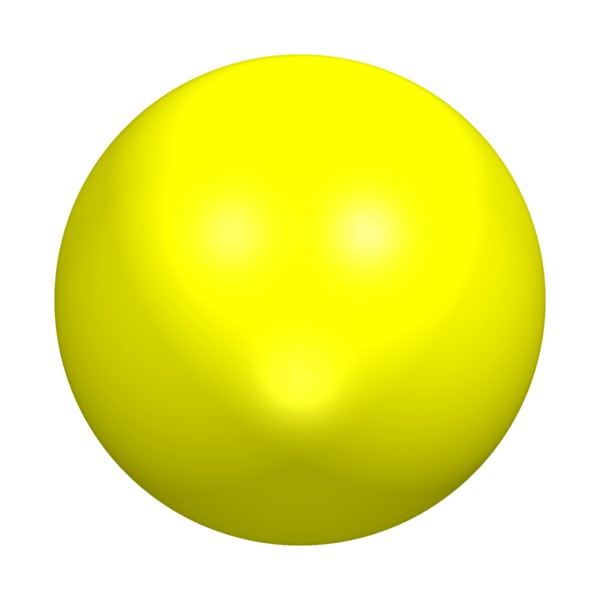
\includegraphics[width=1.1cm]{kugel}
        \end{tabular}
        &
        \begin{tabular}{@{}c@{}}
          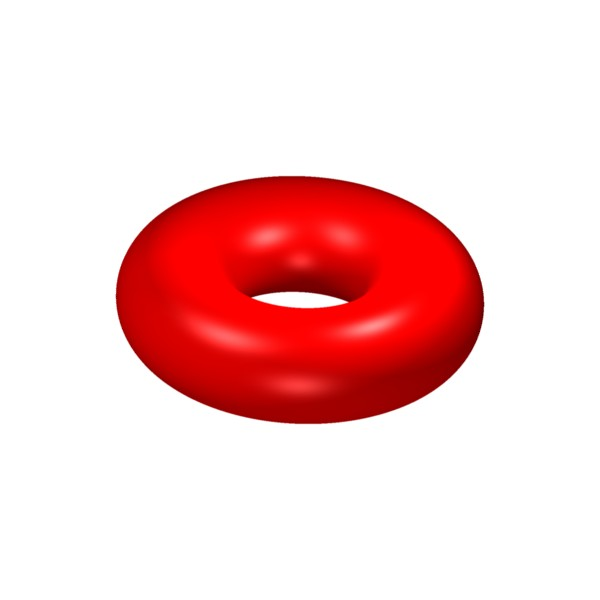
\includegraphics[width=1.1cm]{torus}
        \end{tabular}
        &
        \begin{tabular}{@{}c@{}}
          veel\\
          singulariteiten:
        \end{tabular}
        &
        \begin{tabular}{c@{}@{}}
          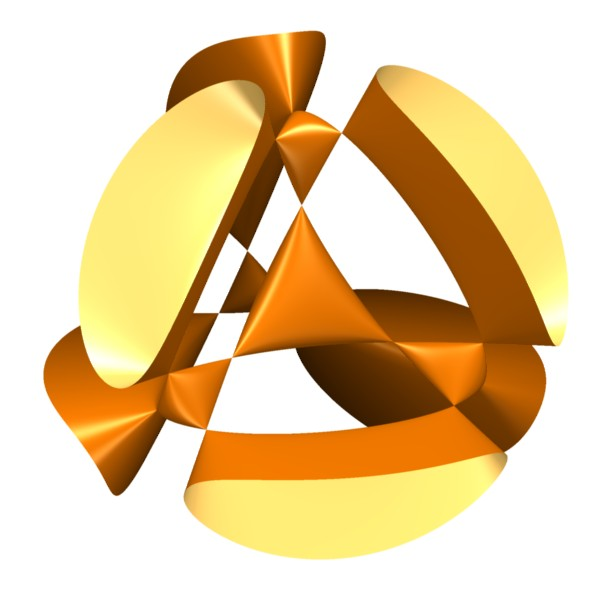
\includegraphics[width=1.1cm]{kummer}
        \end{tabular}
        &
        \begin{tabular}{c@{}@{}}
          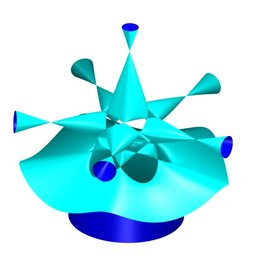
\includegraphics[width=1.1cm]{togliatti}
        \end{tabular}
        &
        \begin{tabular}{c@{}@{}}
          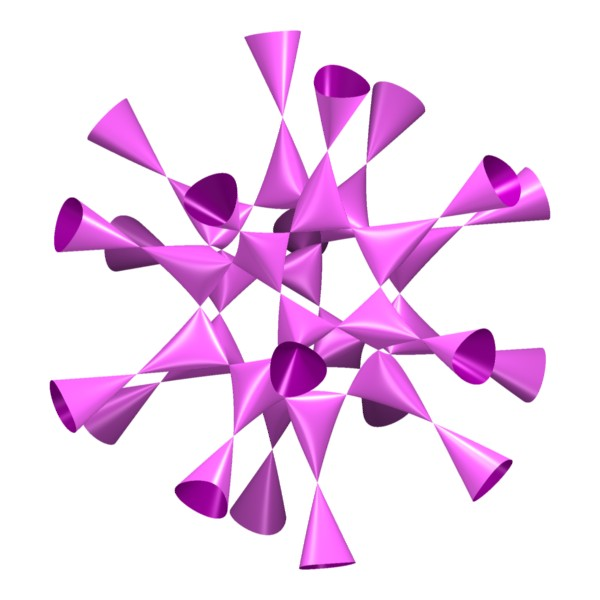
\includegraphics[width=1.1cm]{barth_sextic}
        \end{tabular}
      \end{tabular}
    \end{center}
    \vspace{-0.2cm}
    Het is dus uitzonderlijk dat een oppervlak w\'el singulariteiten heeft, en dit zijn dan ook de meest interessante punten van het oppervlak. De oppervlakken in SURFER worden gedefinieerd door veeltermen. De hoogste macht van een veelterm wordt haar graad $d$ genoemd. Een wiskundig interessante vraag is dan hoeveel singulariteiten een oppervlak van een bepaalde graad maximaal kan hebben.
    We zullen dit getal met $\mu(d)$ aanduiden.

    Nu blijkt dat het getal $\mu(d)$ zeer moeilijk te berekenen is.
    Sinds de 19de eeuw kent men de waarde van $\mu(d)$ voor $d=1,2,3,4$, maar voor $d=5$ werd $\mu(d)$ pas in 1980 gevonden, en voor $d=6$ in 1996.
    Voor $d\geqslant 7$ is de waarde van $\mu(d)$ nog steeds niet gekend.
  
    De oplossing voor algemene waarden van $d$ is nog niet in zicht, en dus is elk nieuw ``record'' voor een bepaalde $\mu(d)$ een belangrijk tussenresultaat.\\  Enkele gekende resultaten:
    
   \begin{center}
      \begin{tabular}{r|cccccccc|c}
        $d$ & $1$ & $2$ & $3$ & $4$ & $5$ & $6$ & $7$ & $8$ & $d$\\
        \hline
        \hline
        \rule{0pt}{1.2em}$\mu(d)\geqslant$ & $0$ & $1$ & $4$ & $16$ & $31$ & $65$ &
        $99$ & $168$ & 
        $\approx \frac{5}{12}d^3$\\[0.3em]
        \hline
        \rule{0pt}{1.2em}$\mu(d)\leqslant$ & $0$ & $1$ & $4$ & $16$ & $31$ & $65$ &
        $104$ & $174$ & $\approx \frac{4}{9}d^3$
      \end{tabular}
    \end{center}
\end{surferIntroPage}
